\documentclass[aspectratio=169,11pt,hyperref={colorlinks=true}]{beamer}
\usepackage[utf8]{inputenc}
\usepackage[T1]{fontenc}
\usepackage{fontspec}
\usepackage[absolute,overlay]{textpos}
\usepackage{listingsutf8}
\usepackage{listings-golang}
\usepackage{tikz}
\usepackage{color}
\usepackage{fontawesome5}
\usepackage{svg}


\title{From Zero to CD with Tekton}
\date[17 Nov 2021 IBM Community Festival]{17 Nov 2021 | \faTwitter ~@blackchip76 | \faGithub ~afrittoli}
\author[Andrea Frittoli]{%
  Andrea Frittoli \\
  Developer Advocate \\
  andrea.frittoli@uk.ibm.com \\
}

\usetheme{af}

% Code style
\setlststyle

\lstdefinelanguage{koyaml}{
  keywords={github, com, afrittoli, examples, ms, go, helloworld},
  sensitive=false,
  comment=[l]{\#},
  morestring=[b]',
  morestring=[b]"
}

% Automatic section frame
% \AtBeginSection{\frame{\sectionpage}}

\begin{document}

\begin{frame}
\titlepage{}
\end{frame}

\begin{lpicrblack}[chewy-I-rgDPLKogs-unsplash.jpg]{%
  Photo by \href{https://unsplash.com/@chewy}{\underline{Chewy}}, CC0
  }%
  {%
  \tableofcontents
  }%
  {}
  \frametitle{Agenda}
\end{lpicrblack}

\section[Introduction]{Introduction}

\begin{sectionwithpic}[mike-benna-X-NAMq6uP3Q-unsplash.jpg]{Photo by \href{https://unsplash.com/@mbenna}{\underline{Mike Benna}}, CC0}
\end{sectionwithpic}

\begin{stripedframe}%
  {%
  Tekton is an open-source framework \\ for creating CI/CD systems \\ ~
  }%
  {%
  Cloud Native \\
  \vspace{0.03\textheight}
  Serveless, Scalable Pipelines \\
  \vspace{0.1\textheight}
  \centering
  \includesvg[width=0.08\paperwidth]{img/tekton-icon-white.svg}
  }%
  {%
  Standardization \\
  \vspace{0.03\textheight}
  Built In Best Practices \\
  \vspace{0.03\textheight}
  Maximum Flexibility \\
  }%
  {%
  Projects \\
  \vspace{0.01\textheight}
  \begin{itemize}
    \item Pipeline
    \item Triggers
    \item Dashboard
    \item CLI
    \item Catalog, Hub
    \item Results
    \item Chains
    \item Operator
  \end{itemize}
  }%
  {%
  Community \\
  \vspace{0.03\textheight}
  More than 150 Companies \\
  \vspace{0.01\textheight}
  Google, IBM, RedHat, VMWare
  }%
  % \begin{textblock*}{0.13\paperwidth}(0.73\paperwidth,0.65\paperheight)
  %   \includesvg[width=0.13\paperwidth]{img/tekton-icon-color.svg}
  % \end{textblock*}
  % A brief into to Tekton
\end{stripedframe}

\note{
  Tekton is an open-source framework for creating continuous delivery systems (aka CI/CD).
  Tekton is built on top of Kubernetes, and it brings all the cloud-native
  advantages into the CD space: serverless execution, scalability and integration with
  the impressive ecosystem of cloud native tools for logging, monitoring, policy enforcement
  and more.

  Tekton has a very small footprint, which makes it easy to get started with it in your minikube
  or kind cluster. That also means having a small control plan overhead when running
  hundres of pipelines. Tekton particuarly shines in large scale CD environments, as it gives
  DevOps architects the full flexibility they need to setup up a CD system which meets the
  enterprise needs for security and compliance, while letting software engineers quickly and
  easily develop their pipelines through a catalog of curated bulding blocks.

  Tekton benefits from a lively community, with contributions from more than 150 companies
  and a collection of different projects that provide from workflow definition, event handling,
  user interfaces, catalog and security.
}

\begin{lgrayrwhiteframe}
  \frametitle{At a Glance}
  \vspace{0.03\paperheight}
  ~~~~~~~~~~~~~~~\includesvg[width=0.1\paperwidth]{img/cdf-stacked-color.svg}
  \vspace{0.03\paperheight}
  ~
  \begin{itemize}
    \item Extend the k8s API with CRDs
    \item Definitions: Task, Pipeline
    \item Execution: TaskRun, PipelineRun
    \item Bindings: \\Workspaces, Parameters, Results
  \end{itemize}
  ~
  \begin{itemize}
    \item Tekton v1 -- Q1 2022
    \item Standalone or building block
  \end{itemize}
  \begin{textblock*}{0.51\paperwidth}(0.48\paperwidth,0.33\paperheight)
    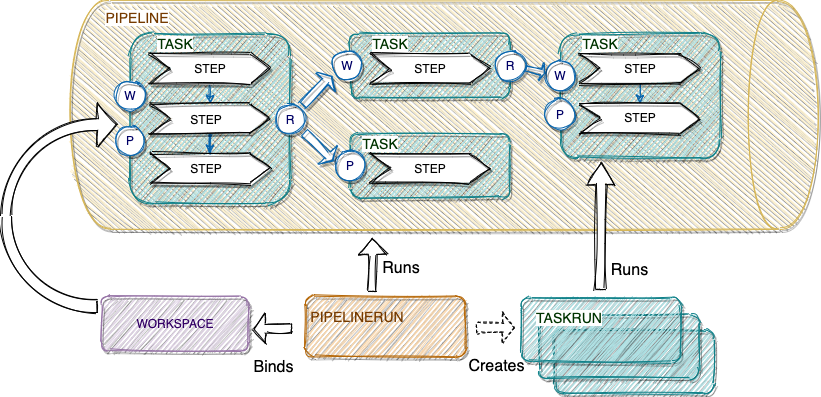
\includegraphics[width=0.5\paperwidth]{img/tekton-workspaces.png}
  \end{textblock*}
\end{lgrayrwhiteframe}

\note{
  Tekton was one of the founding members of the continuous delivery foundation (CDF)
  back at the beginning of 2019.
  It extends the k8s API with CD specific resources.
  Tasks, Pipelines...
  We aim for the Q1 or 2022 for Tekton v1
  Tekton is often used as building block for other platforms, like OpenShift Pipelines,
  Jenkins X, Kubeflow Pipelines and more. The Tekton community cares deeply
  about the stability of its API and happiness of its users.
}

\section[From 0 to CD]{From 0 to CD\\\ldots step by step}
\begin{sectionwithpic}[cat-walking-on-stairs.jpg]{Public domain photo, CC0}
\end{sectionwithpic}

\note{
  Let's see Tekton in action.
  For the demo sections today, we'll use OpenShift Pipelines, which is a distribution
  of Tekton nicely integrated in OpenShift.
}

\begin{lpicrblack}[nadi-whatisdelirium-fZ8uf_L52wg-unsplash.jpg]{%
  Photo by \href{https://unsplash.com/@whatisdelirium}{\underline{Nadi Whatisdelirium}}, CC0
  }%
  {%
  \begin{itemize}
    \item One-liner (almost)
    \item Tekton Operator (\href{https://operatorhub.io/operator/tektoncd-operator}{\underline{OperatorHub}})
    \item Nightly Builds (Operator too)
    \item Helm (by CDF)\\~
    \item Multi-architecture (amd64, s390x, ppc64le, arm64)
    \item Multi-OS (Workloads can run on Windows/amd64)
  \end{itemize}
  ~
  \begin{itemize}
    \item \href{https://cloud.redhat.com/learn/topics/ci-cd}{OpenShift Pipelines}
    \item Let's install it!
  \end{itemize}
  }%
  {0.42}%
  \frametitle{~~~~~~~~~~~~~~~~~~~~~~~~~~~~~~~~~~~~~~~~~~~~~~~~~~Install}
\end{lpicrblack}

\note{
  First thing, we need to install Tekton.
  There are several options, from a simple one-liner command with kubectl to
  an operator. Tekton can run on several different architectures. It is also
  possible to run Tekton Tasks on Windows cluster nodes.

  OpenShift supports an operator.
  -> Show installing openshift
}

\begin{lgrayframerpic}[thom-milkovic-FTNGfpYCpGM-unsplash.jpg]{%
  Photo by \href{https://unsplash.com/@thommilkovic}{\underline{Thom Milkovic}}, CC0
  }%
  {%
  \begin{itemize}
    \item Catalog \& Hub
    \item Tasks \& Pipelines
    \item Parameters, Results \& Workspaces
    \item OCI Bundles
  \end{itemize}
  ~
  \begin{itemize}
    \item Let's install some tasks and pipelines
  \end{itemize}
  }%
  {0.48}
  \frametitle{Authoring}
\end{lgrayframerpic}

\note{

}

\begin{lpicrblack}[john-yunker-Z9rKuPEU6Uc-unsplash.jpg]{%
  Photo by \href{https://unsplash.com/@jyunker}{\underline{John Yunker}}, CC0
  }%
  {%
  \begin{itemize}
    \item Running Tasks \& Pipelines
  \end{itemize}
  ~\\
  \begin{itemize}
    \item Tekton Dashboard
    \item \code{tkn}, \code{kubectl}
    \item Pods, Volumes \& Events
  \end{itemize}
  ~
  \begin{itemize}
    \item OpenShift Console
  \end{itemize}
  }%
  {0.50}%
  \frametitle{~~~~~~~~~~~~~~~~~~~~~~~~~~~~~~~~~~~~~~~~~~~~~~~~~~~~~~~~~~~~~Watching}
\end{lpicrblack}


\begin{lgrayframerpic}[pouncing-cat.png]{Public domain photo, CC0}%
  {%
  \begin{itemize}
    \item Tekton Triggers
    \item Setting up a\\Webhook
    \item Filtering with\\Interceptors
    \item Filtering with\\When Expressions
  \end{itemize}
  }%
  {0.30}
  \frametitle{Launching}
\end{lgrayframerpic}

\begin{lpicrblack}[sereja-ris-g3B53PbBfwU-unsplash.png]{%
  Photo by \href{https://unsplash.com/@serejaris}{\underline{Sereja Ris}}, CC0
  }%
  {%
  \begin{itemize}
    \item Unattended Execution
    \item Events, \code{CloudEvents}
    \item Notifications:\\GitHub, Slack and more
    \item Monitoring \& Measuring
  \end{itemize}
  ~\\
  \begin{itemize}
    \item Tekton Results
    \item Resource Cleanups (WIP)
  \end{itemize}
  }%
  {0.65}%
  \frametitle{~~~~~~~~~~~~~~~~~~~~~~~~~~~~~~~~~~~~~~~~~~~~~~~~~~~~~~~~~~~~~~~~~~~~~~~~~~~~~~~~~~~~Monitoring \& Cleanup}
\end{lpicrblack}

\begin{2columnsframe}{Experiments \& Dogfooding}%
  {%
  \begin{itemize}
    \item Custom Tasks:\\
          Loops \& Iterations \\
          Pipeline in Pipelines
          Wait, CEL Run
  \end{itemize}
  ~\\
  ~\\
  ~\\
  ~\\
  \begin{itemize}
    \item Custom Interceptors (GitHub)
    \item DSL, SDK, Notifiers
  \end{itemize}
  }{%
  \begin{itemize}
    \item Using Tekton to CD Tekton
    \item Release, GitOps, CI \\~
  \end{itemize}
  ~\\
  ~\\
  ~\\
  ~\\
  \begin{itemize}
    \item From Experiments to Feature
    \item Source of examples
    \item Bug discovery, feature requests
  \end{itemize}
  }
\end{2columnsframe}

\section[Roadmap]{Roadmap}
\begin{sectionwithpicrx}[julie_falk_flickr_22258190324_6a583208ae_k.png]{Photo by \href{https://www.flickr.com/photos/piper/}{\underline{Julie Falk}}, CC BY-NC 2.0}
\end{sectionwithpicrx}


\begin{2columnsframe}{Roadmap \& Vision}%
  {%
  Mission:
  \begin{itemize}
    \item Be the industry-standard,\\
          cloud-native CI/CD platform \\
          components and ecosystems \\
  \end{itemize}
  ~\\
  ~\\
  \tiny~\\
  \normalsize
  Vision:
  \begin{itemize}
    \item Tekton API conformance across\\
          as many CI/CD platforms as possible
  \end{itemize}
  }{%
  Vision:
  \begin{itemize}
    \item A rich catalog of high quality,\\
          reusable Tasks which work\\
          with Tekton conformant systems\\
  \end{itemize}
  ~\\
  ~\\
  \tiny~\\
  \normalsize
  Roadmap 2021:
  \begin{itemize}
    \item Towards GA
    \item LTS Policies
    \item User stories, Documentation
    \item Dogfooding
  \end{itemize}
  }
\end{2columnsframe}

% \begin{blackframe}
%   \frametitle{TEP (optional)}
%   \begin{itemize}
%     \item Design principles
%     \item TEP process
%     \item TEP table
%   \end{itemize}
% \end{blackframe}

\section[Q\&A]{Thank You! \\Questions?}

\begin{sectionwithpiclargecentral}[carl-jorgensen-5nrnxx_tWe8-unsplash.jpg]{Brecon Beacons, Walse, Photo by \href{https://unsplash.com/@scamartist}{\underline{Carl Jorgensen}}, CC0}
\end{sectionwithpiclargecentral}

\begin{blackframe}
  \frametitle{References}
  \begin{itemize}
    \item \large Come and Join Us at Tekton!
    \item \normalsize Tekton community: \href{https://github.com/tektoncd/community}{github.com/tektoncd/community} \\
  \end{itemize}
  \begin{itemize}
    \item Slides: \href{https://github.com/afrittoli/zero_to_tekton/blob/cnd2021/zero_to_tekton.pdf}{github.com/afrittoli/zero\_to\_tekton}
    \item Tekton: \href{https://tekton.dev}{tekton.dev}
    \item Tekton Docs: \href{https://tekton.dev/docs}{tekton.dev/docs}
    \item Tekton on GitHub: \href{https://github.com/tektoncd}{github.com/tektoncd}
    \item Tekton Hub: \href{https://hub.tekton.dev}{hub.tekton.dev}
    \item Tekton on Operator Hub:\\\href{https://https://operatorhub.io/operator/tektoncd-operator}{https://operatorhub.io/operator/tektoncd-operator}
    \item Tekton Results: \href{https://github.com/tektoncd/results}{github.com/tektoncd/results}
    \item Tekton Enhancement Proposals (TEPs): \href{https://github.com/tektoncd/community/tree/main/teps\#tekton-enhancement-proposals-teps}{github.com/tektoncd/community/tree/main/teps}
  \end{itemize}
  \begin{textblock*}{0.13\paperwidth}(0.73\paperwidth,0.65\paperheight)
    \includesvg[width=0.13\paperwidth]{img/tekton-icon-color.svg}
  \end{textblock*}
\end{blackframe}

\end{document}
